
\section*{Plots obtained}

\begin{figure}[!ht]
    \centering
    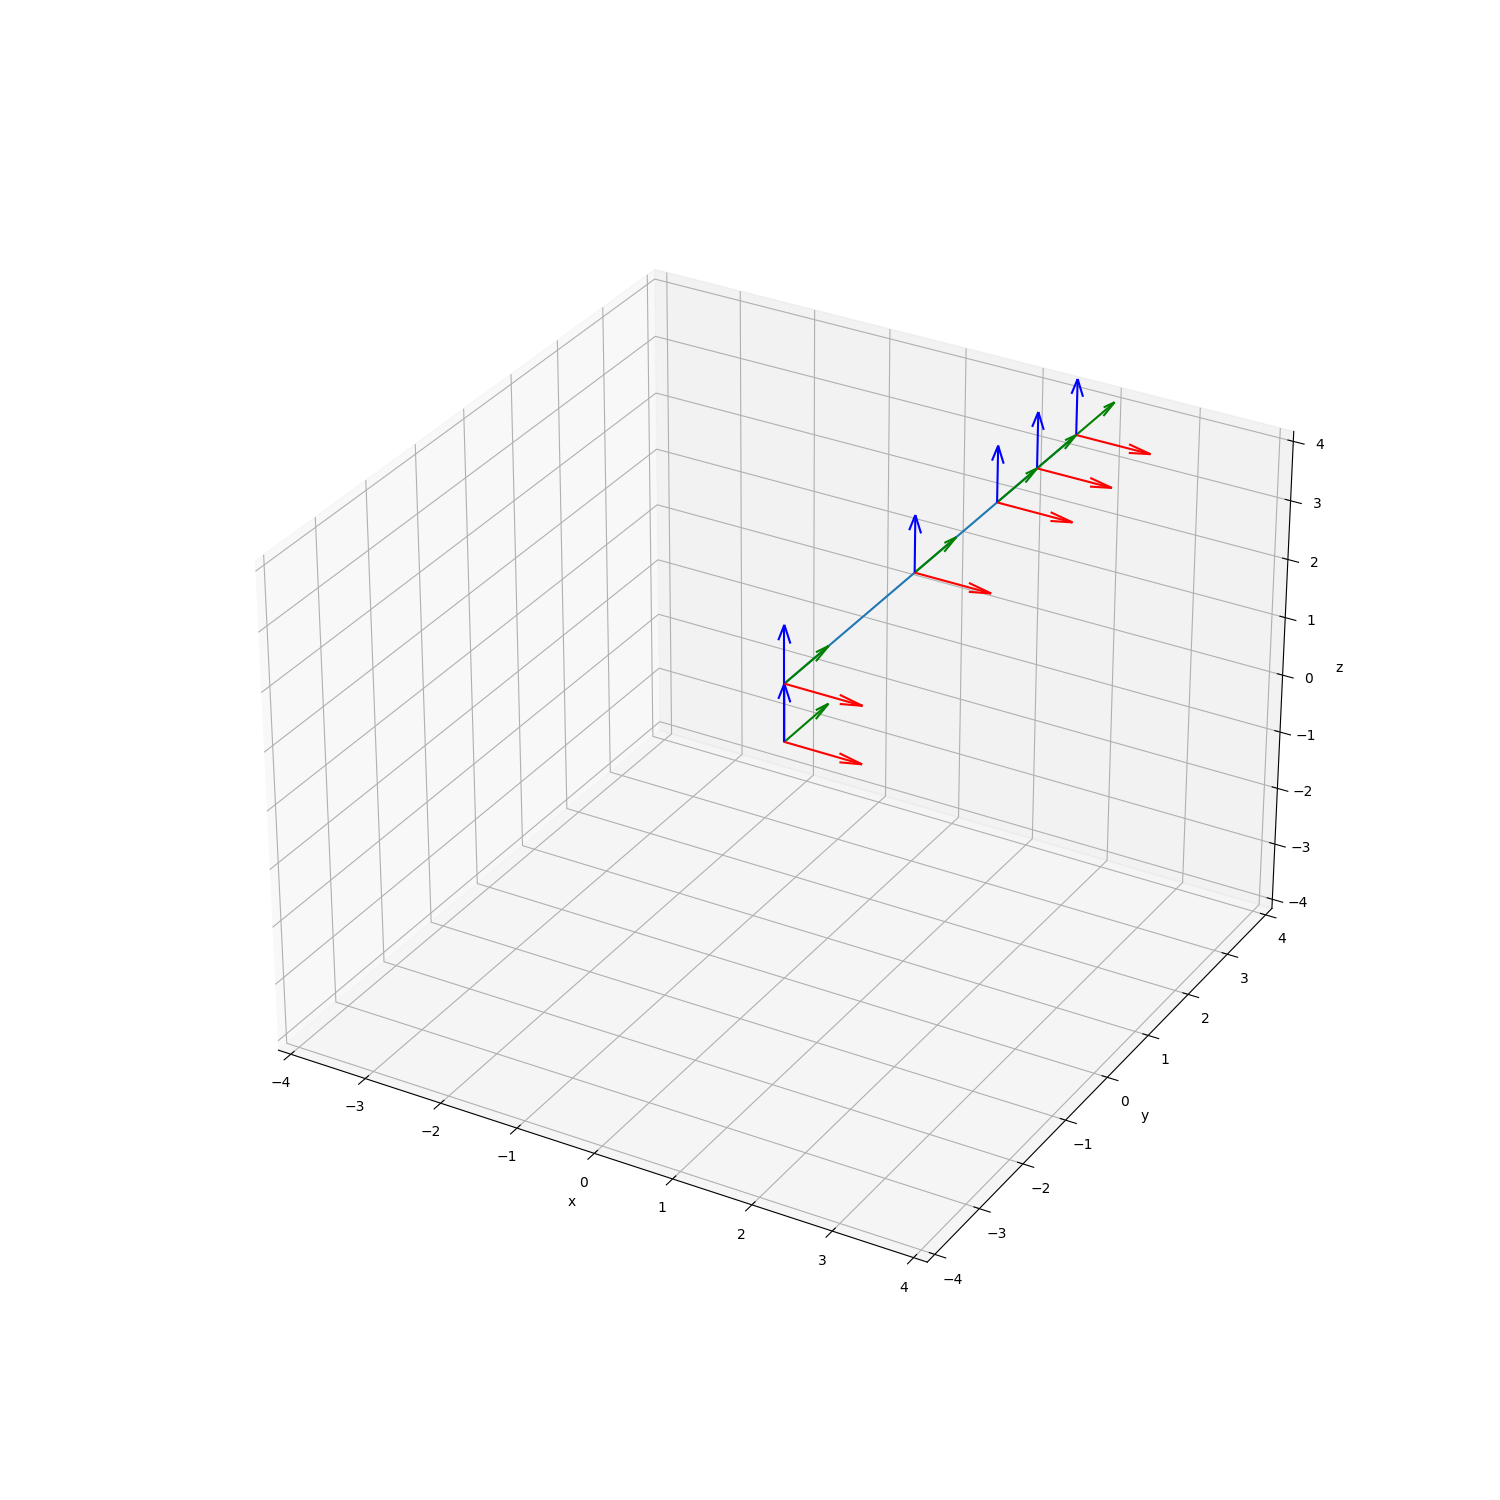
\includegraphics[width=\linewidth]{forward_zeros}
    \caption{Obtained positions for zero angles}
    \label{fig:figure1}
\end{figure}

\begin{figure}[!ht]
    \centering
    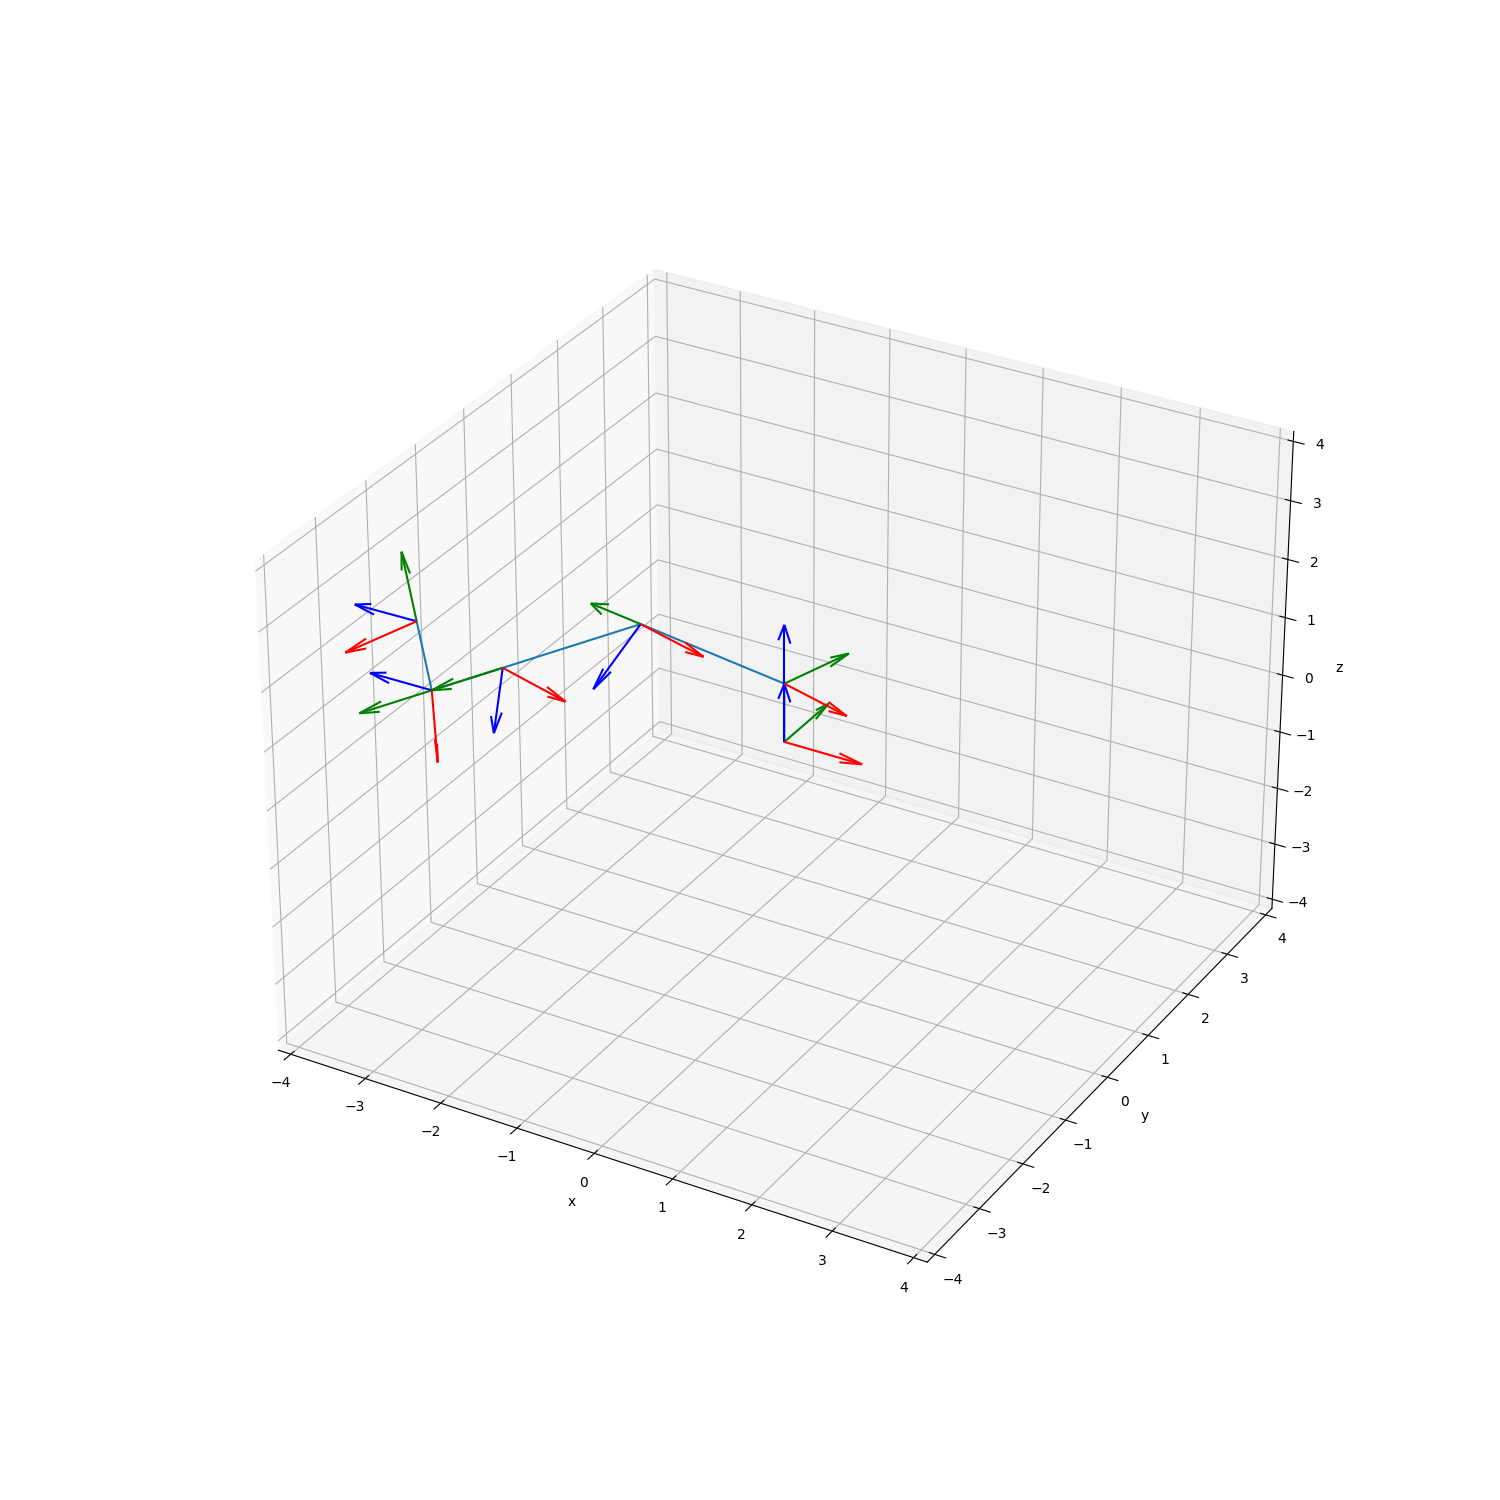
\includegraphics[width=\linewidth]{forward_random}
    \caption{Obtained positions for random angles}
    \label{fig:figure2}
\end{figure}

\begin{figure}[!ht]
    \centering
    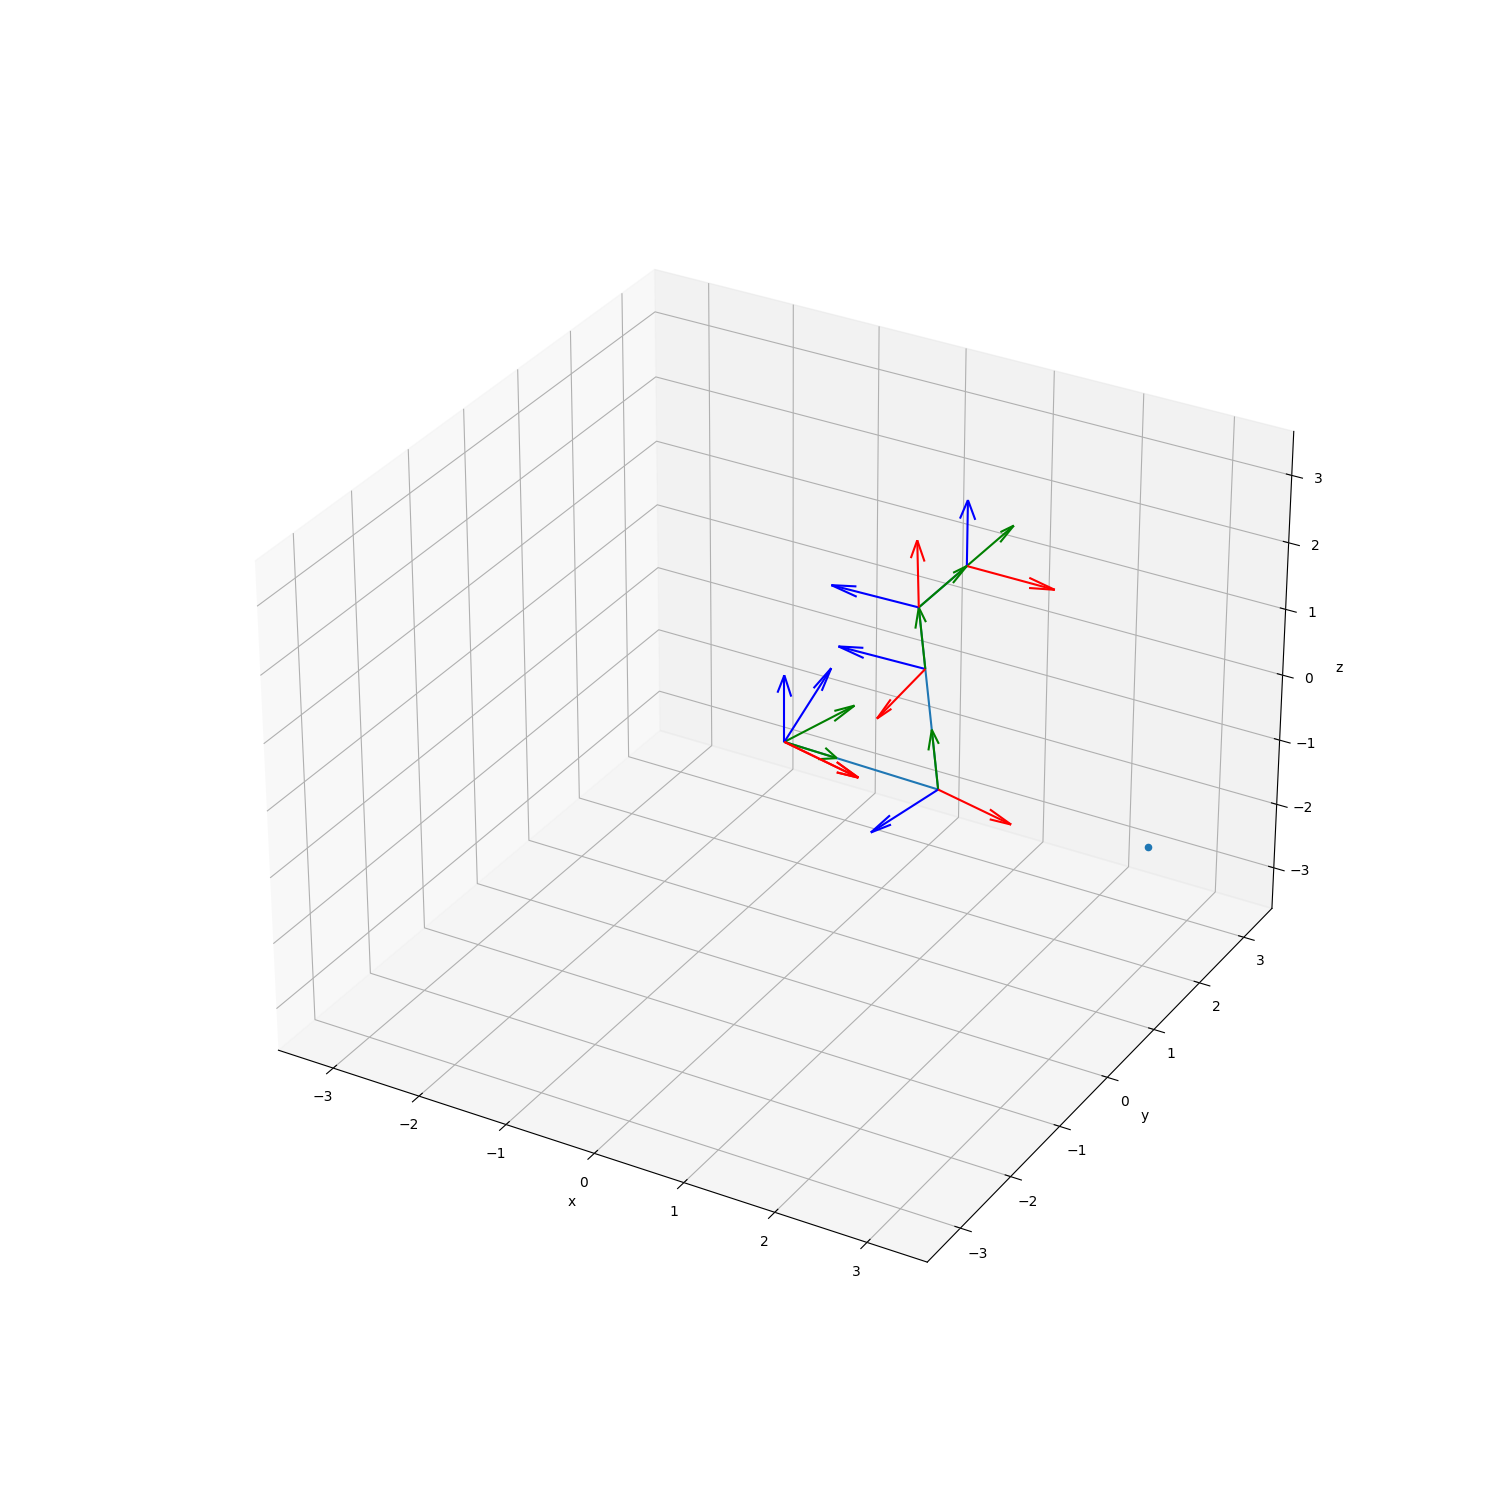
\includegraphics[width=\linewidth]{inverse_example.png}
    \caption{Obtained inverse kinematics for position (4, 0, 0)}
    \label{fig:figure3}
\end{figure}

As you can see on figure 3, manipulator did not reach the desired position (you can see it on figure 3 as blue point), hence the algorithm for inverse kinematics did not work.